%%%%%%%%%%%%%%%%%%%%%%%%%%%%%%%%%%%
%%%  Filename: thesis_template.tex
%%%  ---
%%%  Template for Master Thesis at DTETI UGM   		
%%%  Created using thesisdtetiugm.cls
%%%  --- 
%%%  Written by Canggih Puspo Wibowo
%%%  [canggihpw@gmail.com]
%%%%%%%%%%%%%%%%%%%%%%%%%%%%%%%%%%%

%% Use option "bahasa" or "english" 
%%    to change the basic language used
%% User option "bachelor", "master", or "doctoral"
%% 	  to change the degree
% \documentclass[<bachelor/master/doctoral>,<bahasa/english>]{thesisdtetiugm}
\documentclass[bachelor,bahasa]{thesisdtetiugm}
%======================================
% Information Input
%======================================
% Input author's name and ID number
\author{DAMAR ARBA PRAMUDITYA}{22/501365/PPA/06386}
% Input the thesis' title
\title{AUTENTIKASI MESIN KE MESIN BERBASIS RISIKO PADA KASUS FHIR MENGGUNAKAN RANDOM FOREST}
% Program and the head of the program
\program{Magister Ilmu Komputer}{<<Program coordinator>>}{<<NIP>>}
% Name of department head and NIP
\departmenthead{<<Head of the department>>}{<<NIP>>}
\major{<<Major>>}
\yearsubmit{2024}
\examdate{<<Exam date>>}
% Name of thesis supervisors/promotors
\addsupervisor{Dosen Pembimbing 1, S.T., M.Eng., PhD.}{<<NIP xxxxxx>>}
\addsupervisor{Dosen Pembimbing 2, S.T., M.Eng., PhD.}{<<NIP xxxxxx>>}
%\addsupervisor{<<Supervisor 3>>}{<<NIP>>}
% Name of examiners
%\addexaminer{<<Examiner 1>>}{<<NIP 1>>}
%\addexaminer{<<Examiner 2>>}{<<NIP 2>>}
%\addexaminer{<<Examiner 3>>}{<<NIP 3>>}
%\addexaminer{<<Examiner 4>>}{<<NIP 4>>}
%\addexaminer{<<Examiner 5>>}{<<NIP 5>>}
%\addexaminer{<<Examiner 6>>}{<<NIP 6>>}
%\addexaminer{<<Examiner 7>>}{<<NIP 7>>}
%\addexaminer{<<Examiner 8>>}{<<NIP 8>>}
%\addexaminer{<<Examiner 9>>}{<<NIP 9>>}

%======================================

% correct bad hyphenation here [example]
% \babelhyphenation[<<english/bahasa>>]{op-tical net-works semi-conduc-tor}
%% Uncomment block of code below to disable hyphenation
%\tolerance=1
%\emergencystretch=\maxdimen
%\hyphenpenalty=10000
%\hbadness=10000

\begin{document}
%======================================
% Create cover etc
%======================================

%---- COVER ----
%\printcover{sample/logougm.png}{Pendadaran/Tesis/Ringkasan Tesis*}
\printcover{sample/logougm.png}{Bachelor}
% *Choose one

%---- ENDORSEMENT PAGE ----
% Select endorsement page type. If you want to use your own PDF file,  
% 	use \printendorsementpdf, or if you want to use JPG file, use 
% 	\printendorsementjpg. Otherwise, use \printendorsement.
% 	Choose one only. Comment out unused command(s).
%
\cleardoublepage \phantomsection
\printendorsement
%\printendorsementpdf
%\printendorsementjpg{sample/scanned-endorsement.jpg}

%---- DEDICATION PAGE ----
\cleardoublepage \phantomsection
\chapterstatement{contents/statement/statement}
%\chapterstatementjpg{sample/scanned-statement.jpg}

\cleardoublepage \phantomsection
\chapterdedication{contents/dedication/dedication}

%---- STATEMENT PAGE ----
% Select statement page type. If you want to use your own JPG file,  
%	use \chapterstatementjpg{<your *.jpg file path>}. Otherwise, 
%	use \chapterstatement{contents/statement/statement}.
%	Choose one only. Comment out unused command(s).
%


%---- PREFACE PAGE ----
\cleardoublepage \phantomsection
\chapterpreface{contents/preface/preface}

%======================================
% Create Table of Contents, List of Figures, List of Tables
% <Do not change this part>
%======================================
\cleardoublepage \phantomsection
\thetoc
\onehalfspacing
\tableofcontents
\singlespacing
\cleardoublepage \phantomsection
\thelot
\listoftables
\cleardoublepage \phantomsection
\thelof
\listoffigures

%======================================

%---- NOMENCLATURE PAGE ----
\cleardoublepage \phantomsection
\chapternomenclature{contents/nomenclature/nomenclature}

%---- INTISARI PAGE----
\cleardoublepage \phantomsection
\chapterintisari{contents/abstract/intisari}

%---- ABSTRACT PAGE----
\cleardoublepage \phantomsection
\chapterabstract{contents/abstract/abstract}


%======================================



%======================================
%  MAIN TEXT
%======================================
\startmain
% You can change 
%    the filename and location of the files inputted
\cleardoublepage \phantomsection
\chapter{Pendahuluan}

\section{Latar Belakang}

Dalam sistem kesehatan digital, FHIR \textit{(Fast Healthcare Interoperability
Resources)} telah menjadi standar yang umum digunakan untuk berbagi data medis
antar sistem. Autentikasi mesin ke mesin (M2M) digunakan untuk mengamankan
akses ke data FHIR oleh aplikasi kesehatan dan sistem lainnya. Namun, metode
autentikasi M2M saat ini cenderung kurang adaptif terhadap risiko keamanan yang
berbeda-beda pada setiap transaksi. Hal ini dapat menyebabkan celah keamanan
dan penyalahgunaan data medis oleh pihak yang tidak berwenang.

Untuk mengatasi masalah ini, penelitian sebelumnya telah mengusulkan
penggunaan autentikasi M2M berbasis risiko pada aplikasi online. Namun,
kebanyakan penelitian hanya menggunakan model statistik sederhana atau aturan
heuristik untuk membangun sistem autentikasi M2M berbasis risiko, seperti yang
dilakukan Steinegger dkk. (2016). Hal ini dapat membatasi kemampuan sistem
untuk mengenali ancaman keamanan yang kompleks.

Oleh karena itu, dalam penelitian ini, kami mengusulkan penggunaan metode
machine learning, khususnya Random Forest, untuk membangun sistem autentikasi
M2M berbasis risiko pada sistem FHIR. Dalam penelitian ini, kami akan
membandingkan kinerja sistem autentikasi M2M berbasis risiko menggunakan
Random Forest dengan kondisi sekarang. Kami juga akan mengevaluasi efektivitas
dan efisiensi dari sistem autentikasi M2M berbasis risiko yang diusulkan. Dengan
demikian, penelitian ini diharapkan dapat meningkatkan keamanan dan keandalan
sistem autentikasi M2M pada sistem kesehatan digital berbasis FHIR.


\section{Rumusan Masalah}

Aturan heuristik untuk membangun sistem autentikasi dinilai membatasi
kemampuan sistem untuk mengenali ancaman keamanan yang kompleks seperti \textit{token reply.}


\section{Batasan Masalah}
Agar penelitian ini dapat dilakukan dengan baik, maka perlu dibuat batasan masalah.
Batasan masalah pada penelitian ini adalah:
\begin{enumerate}
	\item Penelitian ini fokus pada mekanisme autentikasi M2M \textit{machine to machine} pada sistem FHIR.
	\item Dataset yang digunakan adalah dataset sintetis login M2M yang dibuat oleh Steinegger dkk. (2016).
	\item Pemilihan fitur dan dataset akan dibatasi dimaksudkan untuk mengurangi kompleksitas model dan keterbatasan sumber daya komputasi.
\end{enumerate}

\section{Tujuan Penelitian}
Tujuan dari penelitian ini adalah:
\begin{enumerate}
	\item Membangun sistem autentikasi M2M berbasis risiko menggunakan Random Forest.
	\item Mengevaluasi kinerja sistem autentikasi M2M berbasis risiko menggunakan Random Forest.
	\item Mengevaluasi efektivitas dan efisiensi sistem autentikasi M2M berbasis risiko menggunakan Random Forest.
	\item Meningkatkan keamanan dan keandalan sistem autentikasi M2M pada sistem kesehatan digital berbasis FHIR.
\end{enumerate}


\section{Manfaat Penelitian}
Manfaat dari penelitian ini adalah diharapkan sebagai berikut:
\begin{enumerate}
	\item Meningkatkan keamanan dan keandalan sistem autentikasi M2M pada sistem kesehatan digital berbasis FHIR.
	\item Menambah pengetahuan dan wawasan mengenai autentikasi M2M berbasis risiko menggunakan Random Forest.
	\item Meminimalisir risiko keamanan pada sistem kesehatan digital berbasis FHIR.
	\item Dapat memodelkan masalah keamanan dengan menggunakan metode machine learning.
\end{enumerate}

\cleardoublepage \phantomsection
\chapter{Tinjauan Pustaka}

Autentikasi berbasis risiko (RBA) adalah metode untuk memverifikasi identitas
pengguna dengan menyesuaikan tingkat autentikasi secara dinamis berdasarkan
tingkat risiko sesi saat ini. Pendekatan ini bertujuan untuk menyeimbangkan
keamanan dan kenyamanan dengan menyediakan langkah-langkah autentikasi yang
lebih kuat ketika tingkat risiko tinggi, dan langkah-langkah yang lebih longgar
ketika tingkat risiko rendah.

Sebuah tinjauan literatur mengenai Autentikasi Berbasis Risiko menemukan
bahwa banyak penelitian telah dilakukan pada topik ini dan berbagai teknik telah
diusulkan. Salah satu teknik yang paling umum adalah menggunakan algoritma
penilaian risiko untuk secara dinamis menyesuaikan tingkat otentikasi berdasarkan
tingkat risiko.

Studi yang dilakukan oleh Thomas dkk. (2017) membahas resiko dari password
yang dicuri dan bagaimana kebocoran kredensial dapat terjadi. Tidak hanya itu
namun studi tersebut juga menampilkan situs situs yang banyak mengalami
kebocoran data. Resiko yang paling besar dapat terjadi adalah data-data kita
disalahgunakan hingga mengalami kerugian material. Sedangkan phising menjadi
faktor utama penyebab terjadinya kebocoran kredensial dan disusul oleh
keyloggers.

Stephan Wiefling dkk. (2022) mengemukakan Risk-Based Authentication
(RBA) dapat memperkirakan apakah login itu sah atau merupakan upaya
pengambilalihan akun. Ini dilakukan dengan memantau dan merekam sekumpulan
fitur yang tersedia dalam konteks login. Fitur potensial berkisar dari jaringan (mis.,
alamat IP), perangkat atau klien (mis., string agen pengguna), hingga informasi
biometrik perilaku (mis., waktu masuk).Selain itu kelebihan RBA juga telah disurvey oleh Cabarcos dkk. (2019)
menganalisis literatur tentang autentikasi adaptif berdasarkan prinsip-prinsip desain
yang terkenal dalam disiplin sistem berbasis resiko dan tantangan nya adalah tidak
ada satu ukuran yang cocok untuk semua dalam keamanan, tidak ada mekanisme baru yang akan menggantikan semua mekanisme lainnya dan diterima sebagai
solusi universal. Doerfler dkk. (2019) menggambarkan bahwa tantangan login
bertindak sebagai penghalang penting untuk pembajakan, tetapi gesekan dalam
proses menyebabkan pengguna yang sah gagal masuk, meskipun pada akhirnya
dapat mengakses akun mereka lagi.

Banyak sistem yang sudah mengimplementasikan RBA karena kelebihannya,
studi yang dilakukan oleh Prasad dkk. (2017) menjadi awal mula bagaimana sistem
perbankan mulai menerapkan autentikasi berdasarkan risiko dengan kombinasi
lokasi. Sedangkan dalam sektor kesehatan sendiri autentikasi standar seperti user
dan password masih banyak digunakan, karena sistem IT kesehatan masih fokus
dalam mengembangkan The Fast Health Interoperability Resources (FHIR) Ayaz
dkk. (2021)

Selanjutnya, beberapa studi dalam literatur mengusulkan metode otentikasi
berbasis risiko yang menggunakan berbagai faktor seperti lokasi, waktu, dan jenis
perangkat untuk menentukan tingkat risiko suatu sesi. Sebagai contoh, sebuah
penelitian oleh Agarwal dkk. (2016) mengusulkan sistem RBA berbasis lokasi yang
menggunakan lokasi perangkat pengguna untuk menentukan tingkat risiko suatu
sesi. Studi ini menemukan bahwa sistem yang diusulkan secara efektif
meningkatkan keamanan sistem dengan tetap mempertahankan kegunaan.

Penggunaan RBA masih terbatas pada major digital service, hal ini sebagian
disebabkan oleh kurangnya pengetahuan dan implementasi terbuka yang
memungkinkan penyedia layanan mana pun untuk meluncurkan perlindungan RBA
kepada penggunanya. Untuk menutup kesenjangan ini, Stephan Wiefling dkk.
(2021) memberikan analisis tentang karakteristik RBA dalam penerapan praktis
sekaligus memberikan dataset yang dapat digunakan secara umum.
Penelitian lain Misbahuddin dkk. (2017) mengusulkan sistem RBA berbasis
perangkat yang menggunakan jenis perangkat dan status perangkat untuk
menentukan tingkat risiko suatu sesi. Penelitian tersebut menemukan bahwa sistem
yang diusulkan secara efektif meningkatkan keamanan sistem dengan tetap
mempertahankan kegunaan menggunakan machine learning.

Penggunaan analisis berbasis risiko dalam konteks machine to machine dibahas
dalam studi yang dilakukan oleh Taneja (2013). Mekanisme keamanan tertentu
mengasumsikan bahwa akhir perangkat sudah diamankan. Dalam jaringan IoT,
perangkat IoT itu sendiri dapat dikompromikan. Seorang penyerang dapat mencuri
perangkat, mendapatkan akses mengaksesnya dan menggunakannya untuk
serangan yang lebih merusak.

Roy dan Dasgupta (2018) sudah meneliti bahwa fuzzy dapat menjadi terobosan
dalam menentukan multifaktor autentikasi. Selain itu, banyak penelitian juga telah
mengusulkan penggunaan algoritma pembelajaran mesin seperti pohon keputusan,
Random Forest, dan jaringan syaraf untuk meningkatkan kinerja RBA. Sebagai
contoh, sebuah penelitian oleh Zhang, F dkk. (2012) mengusulkan sistem RBA
yang menggunakan algoritma Random Forest untuk menentukan tingkat risiko dari
sebuah sesi. Penelitian ini menemukan bahwa sistem yang diusulkan mencapai
tingkat akurasi yang tinggi dan meningkatkan keamanan sistem. Dalam studi lain
Alam dan Vuong (2013), Speiser dkk. (2019) menunjukkan bahwa Random Forest
adalah pilihan yang baik karena dapat secara efektif mengklasifikasikan transaksi
berdasarkan tingkat resikonya menggunakan serangkaian fitur yang berasal dari
data transaksi. Random Forest adalah algoritma pembelajaran mesin yang kuat yang
dapat menangani kumpulan data besar dan mampu menangani kebisingan dan nilai
yang hilang dengan baik. Selain itu, dapat memberikan skor kepentingan fitur, yang
dapat digunakan untuk mengidentifikasi fitur yang paling penting untuk klasifikasi
risiko. Secara keseluruhan, Random Forest adalah algoritma pembelajaran mesin
yang efektif dan banyak digunakan untuk otentikasi M2M berbasis risiko.

Rangkuman penelitian sebelumnya dapat dilihat pada Tabel 2.1. Dalam studi
ini ditawarkan pendekatan autentikasi berbasis risiko dengan menggunakan dalam
kasus machine to machine device yang dikaitkan dalam FHIR service.

% todo: tabel 2.1


\cleardoublepage \phantomsection
\chapter{Landasan Teori}

\section{FHIR (Fast Healthcare Interoperability Resources)}
FHIR, singkatan dari Fast Healthcare Interoperability Resources, merupakan standar internasional yang diperkenalkan oleh Health Level Seven International (HL7) untuk memfasilitasi pertukaran data kesehatan elektronik. Standar ini dirancang untuk mengatasi tantangan interoperabilitas antara sistem-sistem informasi kesehatan yang beragam, dengan tujuan memungkinkan pertukaran data yang cepat, fleksibel, dan terstandarisasi di seluruh industri kesehatan. 

FHIR menggunakan format data yang ringan seperti JSON atau XML, dan protokol komunikasi web standar seperti HTTP atau HTTPS, yang memfasilitasi integrasi dengan sistem-sistem modern dengan lebih mudah. Dengan pendekatan moduler, FHIR memungkinkan akses granular terhadap informasi kesehatan, sesuai kebutuhan aplikasi atau pengguna. 

Adopsi FHIR diharapkan dapat meningkatkan interoperabilitas di seluruh rantai perawatan kesehatan, memungkinkan pertukaran informasi yang lebih efisien dan akurat, serta mendukung pengembangan aplikasi kesehatan yang inovatif dan terintegrasi. Sebagai hasilnya, FHIR juga membuka pintu bagi pengembangan solusi-solusi teknologi kesehatan yang lebih canggih, seperti analisis big data dan kecerdasan buatan, serta integrasi dengan perangkat medis wearable.

\section{Autorisasi}
Otorisasi merujuk pada proses yang menentukan hak akses yang diberikan kepada entitas setelah autentikasi identitasnya berhasil dilakukan. Otorisasi memainkan peran penting dalam mengatur akses ke sumber daya dan layanan di dalam suatu sistem. Ini melibatkan penentuan apakah subjek atau entitas memiliki izin yang sesuai untuk melakukan tindakan tertentu dalam lingkungan yang diberikan. Proses otorisasi sering kali dilakukan setelah proses autentikasi yang sukses, di mana autentikasi memverifikasi identitas entitas. Dengan adanya otorisasi, sistem dapat memastikan bahwa hanya entitas yang memiliki hak yang sesuai yang diberikan akses ke sumber daya atau layanan tertentu, yang pada gilirannya membantu menjaga keamanan sistem secara keseluruhan. Misalnya, dalam sebuah aplikasi perbankan, setelah seorang pengguna berhasil mengautentikasi identitasnya, proses otorisasi akan menentukan hak akses pengguna tersebut terhadap fungsi-fungsi seperti pengecekan saldo, transfer dana, atau pembayaran tagihan. Oleh karena itu, pemahaman yang mendalam tentang konsep otorisasi penting untuk merancang dan mengimplementasikan sistem informasi yang aman dan efektif.

\section{Autentikasi}
Autentikasi adalah konsep fundamental yang diperlukan untuk memvalidasi keaslian identitas entitas tertentu dalam suatu sistem. Identitas, sebagai inti dari autentikasi, merujuk pada informasi yang digunakan untuk mengidentifikasi subjek. Kredensial, sebagai elemen kunci dalam proses autentikasi, terdiri dari informasi otentikasi yang diperlukan untuk membuktikan identitas subjek, seperti kata sandi, token, atau biometrik.

Metode autentikasi beragam dan dapat mencakup kata sandi, token, biometrik, sertifikat digital, serta otorisasi multi-faktor (MFA). Protokol autentikasi, sebagai serangkaian langkah atau aturan, memberikan panduan bagi pelaksanaan autentikasi dalam suatu sistem, contohnya OAuth, OpenID, SAML, dan Kerberos.

Keamanan merupakan aspek krusial dalam autentikasi, yang mencakup kerahasiaan kredensial, integritas data autentikasi, dan non-repudiasi. Pemahaman akan kelemahan dan ancaman terhadap sistem autentikasi, seperti serangan phishing, brute force, dan man-in-the-middle, penting untuk meningkatkan ketahanan sistem.

Selain itu, autentikasi harus dapat diandalkan, sehingga sistem dapat memberikan verifikasi identitas yang konsisten dan akurat

\subsection{Standar Autentikasi pada FHIR}
Hubungan antara autentikasi dan FHIR berkaitan dengan keamanan dan akses kontrol dalam pertukaran data kesehatan elektronik. Autentikasi digunakan untuk memverifikasi identitas entitas yang terlibat dalam pertukaran data menggunakan standar FHIR. Setelah identitas tersebut diverifikasi, otorisasi diterapkan untuk menentukan hak akses entitas tersebut terhadap data yang disediakan oleh layanan FHIR.

Dalam konteks FHIR, autentikasi digunakan untuk memastikan bahwa entitas yang mencoba mengakses atau menyediakan data kesehatan melalui API FHIR adalah entitas yang sah. Ini bisa berarti memverifikasi identitas pengguna, aplikasi, atau sistem yang berusaha berinteraksi dengan layanan FHIR. Autentikasi bisa dilakukan menggunakan berbagai metode, seperti kata sandi, token, atau mekanisme autentikasi yang lebih kuat seperti sertifikat digital atau biometrik, tergantung pada kebutuhan dan kebijakan keamanan sistem.

Setelah autentikasi berhasil dilakukan, otorisasi diterapkan untuk menentukan apa yang diizinkan entitas tersebut lakukan dengan data yang tersedia melalui layanan FHIR. Misalnya, seorang dokter mungkin memiliki akses penuh untuk melihat dan mengubah catatan medis pasien tertentu, sementara seorang petugas administrasi hanya diizinkan untuk melihat informasi dasar pasien tanpa memiliki kemampuan untuk mengubahnya. Otorisasi dalam konteks FHIR memastikan bahwa akses ke data kesehatan dikontrol sesuai dengan kebutuhan dan kebijakan privasi yang berlaku.

Dengan demikian, autentikasi dan otorisasi berperan penting dalam menjaga keamanan dan kerahasiaan data kesehatan yang ditangani oleh layanan FHIR, memastikan bahwa hanya entitas yang berwenang yang dapat mengakses informasi yang sensitif dan penting tersebut.

\subsection{Autentikasi Mesin ke Mesin}
Machine-to-Machine (M2M) authentication adalah proses verifikasi yang digunakan untuk mengautentikasi perangkat atau mesin yang terhubung ke jaringan, seperti komputer, perangkat IoT, atau perangkat mobile. Proses ini memastikan bahwa hanya perangkat yang sah yang dapat terhubung ke jaringan dan mengakses data atau layanan yang tersedia seperti skema pada Gambar \ref*{fig:m2m}.

M2M authentication dapat menggunakan berbagai metode, seperti pengenalan suara, pengenalan wajah, pengenalan sidik jari, atau kombinasi dari metode tersebut. Dalam beberapa kasus, M2M authentication juga dapat menggunakan teknologi kriptografi, seperti enkripsi atau sertifikat digital, untuk memastikan keamanan komunikasi antar perangkat.
\begin{figure}
    \centering
    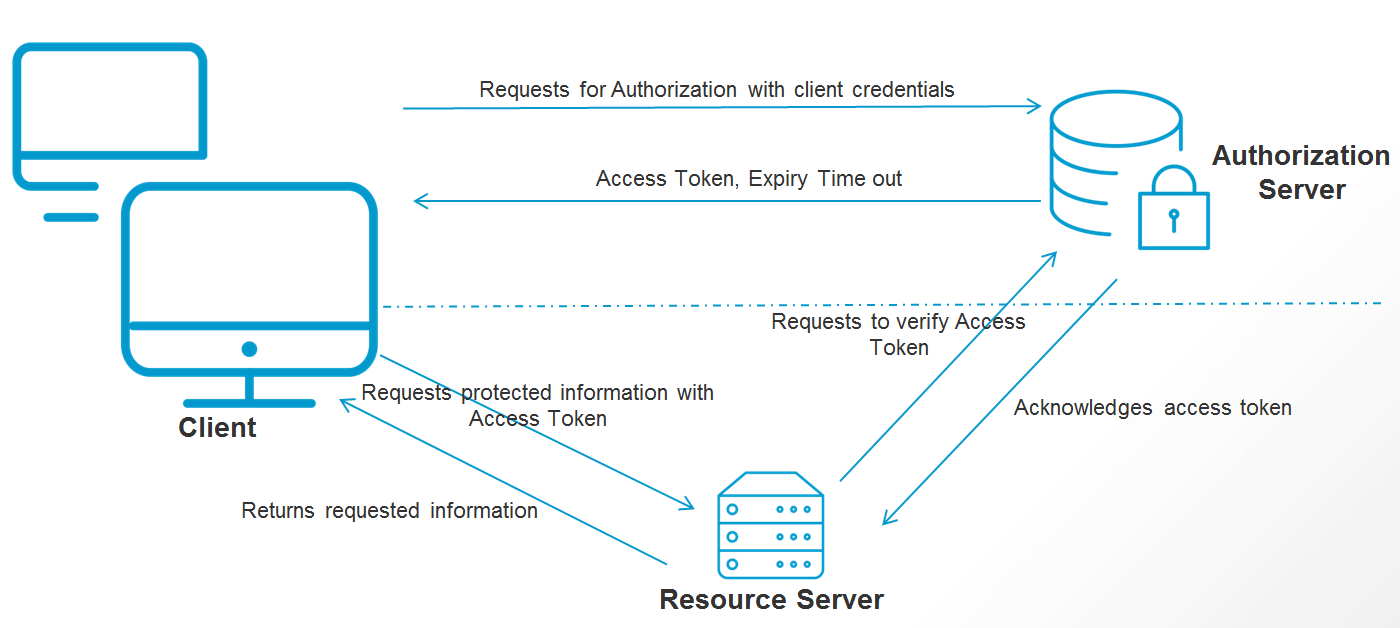
\includegraphics[width=0.8\textwidth]{contents/chapter-3/m2m_auth.png}
    \caption{Skema M2M Authentication}
    \label{fig:m2m}
\end{figure}

M2M authentication juga dapat digabungkan dengan metode risk-based authentication untuk meningkatkan keamanan sistem. Dengan menganalisis faktor- faktor yang dapat meningkatkan risiko, seperti lokasi geografis, waktu akses, dan jenis perangkat yang digunakan, sistem dapat mengambil tindakan yang sesuai untuk menangani ancaman potensial.

\subsection{Metode Autentikasi M2M}
Salah satu metode autentikasi Machine-to-Machine (M2M) menggunakan token merujuk pada proses verifikasi identitas antara dua atau lebih perangkat atau sistem tanpa intervensi manusia. Dalam skenario ini, token digunakan sebagai kredensial atau kunci otentikasi yang diberikan kepada perangkat atau sistem untuk membuktikan identitasnya kepada sistem yang lain.

\subsubsection{Token}
Klien membuat permintaan ke server otorisasi dengan mengirimkan ID klien, rahasia klien, bersama dengan audiens dan klaim-klaim lainnya. Server otorisasi memvalidasi permintaan tersebut, dan, jika berhasil, mengirimkan respons dengan token akses. Klien sekarang dapat menggunakan token akses untuk meminta sumber daya yang dilindungi dari server sumber daya.
Karena klien harus selalu menjaga rahasia klien, pemberian ini hanya dimaksudkan untuk digunakan pada klien terpercaya. Dengan kata lain, klien yang menyimpan rahasia klien harus selalu digunakan di tempat di mana tidak ada risiko rahasia tersebut disalahgunakan. Sebagai contoh, meskipun mungkin ide yang baik untuk menggunakan hibah kredensial klien di sistem internal yang mengirimkan laporan di seluruh web ke bagian lain dari sistem Anda, namun tidak dapat digunakan untuk alat publik yang dapat diakses oleh pengguna eksternal mana pun.
Berikut ini adalah permintaan HTTP yang relevan pada Tabel \ref{tab:req_http} berikut:

\begin{table}[H]
    \caption{Permintaan HTTP}
    \vspace{0.5em}
    \centering
    \begin{tabular}{|c|c|c|}
        \hline
        Permintaan & Deskripsi \\
        \hline \hline
        POST & Metode HTTP \\
        \hline
        /token & Endpoint \\
        \hline
        grant\_type=client\_credentials & Jenis hibah \\
        \hline
        & ID klien \\
        \hline
        & Rahasia klien \\
        \hline
        & Audiens \\
        \hline
    \end{tabular}
    \label{tab:req_http}
\end{table}

Sedangkan berikut contoh respon HTTP yang relevan pada Tabel \ref{tab:res_http} berikut:

\begin{table}[h]
    \caption{Respon HTTP}
    \vspace{0.5em}
    \centering
    \begin{tabular}{|c|c|c|}
        \hline
        Respon & Deskripsi \\
        \hline \hline
        200 OK & Kode status HTTP \\
        \hline
        Content-Type: application/json & Header HTTP \\
        \hline
        Cache-Control: no-store & Header HTTP \\
        \hline
        Pragma: no-cache & Header HTTP \\
        \hline
        \{ & Body \\
        \hline
        "access\_token": "2YotnFZFE & \\
        \hline
        "token\_type": "example", & \\
        \hline
        "expires\_in": 3600, & \\
        \hline
        "example\_parameter": "example\_value" & \\
        \hline
        \} & \\
        \hline
    \end{tabular}
    \label{tab:res_http}
\end{table}

\section{\textit{Risk Based Authentication}}
Risk-based adalah suatu metode yang digunakan untuk mengukur dan
mengelola risiko. Dalam konteks keamanan, risk-based authentication adalah metode autentikasi yang mengukur tingkat risiko dari suatu permintaan akses, dan mengambil tindakan yang sesuai berdasarkan tingkat risiko tersebut. Metode ini bertujuan untuk mengenali dan menangani ancaman potensial tanpa mengekang fleksibilitas dan kenyamanan pengguna.
Dalam konteks Machine-to-Machine (M2M) authentication, risk-based authentication digunakan untuk mengukur tingkat risiko dari suatu permintaan akses dan mengambil tindakan yang sesuai berdasarkan tingkat risiko tersebut.
Prosesnya dapat dilakukan dengan cara menganalisis faktor-faktor yang dapat meningkatkan risiko, seperti lokasi geografis, waktu akses, dan jenis perangkat yang digunakan.
Setelah tingkat risiko diukur, sistem dapat mengambil tindakan yang sesuai. Jika tingkat risiko dianggap rendah, maka autentikasi dapat dilakukan secara otomatis tanpa intervensi manusia. Namun, jika tingkat risiko dianggap tinggi, maka autentikasi dapat dilakukan dengan cara yang lebih ketat, seperti mengharuskan verifikasi melalui kode SMS atau panggilan telepon, atau pembatasan akses sesuai dengan level risiko.
Risk-based authentication juga dapat digabungkan dengan metode analisis risiko dinamis, yaitu mengukur risiko secara real-time dan mengambil tindakan sesuai dengan situasi yang ada. Ini dapat membantu sistem untuk mengenali dan menangani ancaman potensial secara efektif tanpa mengekang fleksibilitas dan kenyamanan pengguna seperti ilustrasi pada Gambar 3.2.

Bagian ini membahas pertimbangan etis penelitian dan [potensi] masalah serta
keterbatasannya. Jika menyangkut penelitian dengan makhluk hidup, maka dibutuhkan adanya \textit{ethical clearance}, di bagian ini hal itu akan dibahas. Demikian juga tentang keterbatasan ataupun masalah yang akan timbul.

\section{\textit{Classification and Regression Tree (CART)}}
Metode CART merupakan suatu metode pohon keputusan (decision tree) yang bersifat recursive partitioning. Satu tree terdiri atas tiga komponen utama yaitu root node, internal node dan terminal node. Pada metode CART simpul akar (root node) dipartisi menjadi dua simpul anak (internal node), masing-masing simpul anak kemudian dipartisi menjadi dua simpul anak yang baru hingga menjadi terminal node yang bersifat homogen sebagai interpretasi dari tree Zhang, H \& Singer (2010). CART membentuk tree dengan dua langkah yaitu, pembentukan maksimal dari decision tree berdasarkan proses splitting (pemilahan) dan pemangkasan (pruning) dengan mempertimbangkan tree dan cabang pohon yang terbentuk. Proses splitting variabel pada percabangan node pada tree dilihat dari variabel yang memiliki nilai goodness of split maksimal. Nilai ini dilihat berdasarkan perubahan gini impurity/gini index pada node t dan percabangan nodenya menurut Gordon dkk. (1984) dengan rumus sebagai berikut.
%insert equation
\\
Node Kiri:
\begin{equation}
    \text{imp}(\mathbf{t}_{\text{L}}) = \sum_{l=1}^{2} p_{\text{tL}}(l)(1 - p_{\text{tL}}(l))
\end{equation}
\\
Node Kanan:
\begin{equation}
    \text{imp}(\mathbf{t}_{\text{R}}) = \sum_{l=1}^{2} p_{\text{tR}}(l)(1 - p_{\text{tR}}(l))
    \end{equation}
\\ 
Node t:
\begin{equation}
    \text{imp}(\mathbf{t}) = \sum_{k=1}^{2} p_{\text{t}}(k)(1 - p_{\text{t}}(k))
    \end{equation}
\\
Keterangan:
\begin{equation}
    p_{t}(k) = \frac{n_{t}(k)}{n_{t}} \quad \text{dan} \quad p_{t}(l) = \frac{n_{t}(l)}{n_{t}}
    \end{equation}
\\
\begin{equation}
    p_{t}(k), p_{t}(l) : \text{Proporsi objek kelas klasifikasi ke-} k \text{ atau ke-} l \text{ pada node } t
    \end{equation}
    
    \begin{equation}
    n_{t}(k), n_{t}(l) : \text{Jumlah observasi kelas klasifikasi ke-} k \text{ atau ke-} l \text{ pada node } t
    \end{equation}
    
    \begin{equation}
    n_{t} : \text{Jumlah seluruh observasi pada node } t
    \end{equation}
    

Gini Impurity berfungsi untuk menentukan seberapa banyak pemisah yang akan dibentuk decision tree. Sementara dalam pemilihan variabel s yang digunakan untuk memilah ditentukan oleh nilai Goodness of Split sebagai berikut.
%insert equation
\begin{equation}
    \Delta\text{imp}(\mathbf{s}, \mathbf{t}) = \text{imp}(\mathbf{t}) - \text{p}_{t\text{L}}\text{imp}(\mathbf{t}_{\text{L}}) - \text{p}_{t\text{R}}\text{imp}(\mathbf{t}_{\text{R}})
    \end{equation}
Keterangan:
\begin{equation}
    p_{t\text{L}} = \frac{n_{t\text{L}}}{n_{t}} \quad \text{and} \quad p_{t\text{R}} = \frac{n_{t\text{R}}}{n_{t}}
    \end{equation}
\\
\begin{equation}
    p_{t}(\text{L atau R}) : \text{Proporsi objek pada node } t \text{ yang memilah pada node } t_{\text{L}} \text{ atau node } t_{\text{R}}
    \end{equation}
    
    \begin{equation}
    n_{t}(\text{L atau R}) : \text{Jumlah observasi pada node } t \text{ yang memilah pada node } t_{\text{L}} \text{ atau node } t_{\text{R}}
    \end{equation}
    
    \begin{equation}
    n_{t} : \text{Jumlah seluruh observasi pada node } t
    \end{equation}
    
Variabel pemilah s yang memiliki goodness of split maksimal merupakan variabel yang lebih baik digunakan untuk melakukan proses splitting. Serta apabila terminal node yang terbentuk dari internal node memiliki nilai gini index lebih besar maka sebaiknya proses splitting dihentikan pada internal node sehingga menjadi terminal node.

\subsection{Random Forest}
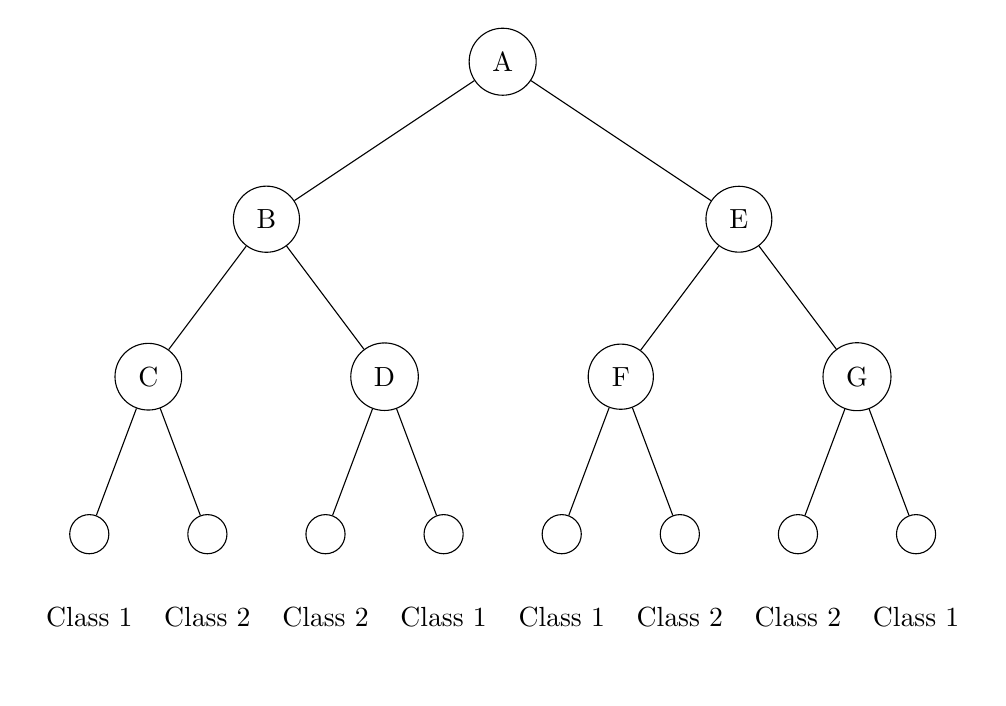
\begin{tikzpicture}[
    grow=down,
    level 1/.style={sibling distance=6cm, level distance=2cm},
    level 2/.style={sibling distance=3cm, level distance=2cm},
    level 3/.style={sibling distance=1.5cm, level distance=2cm},
    every node/.style={draw, circle, inner sep=0.5em}
  ]
  
  % Root node
  \node {A}
    child {
      node {B}
      child {
        node {C}
        child {node[label=below:Class 1] {}}
        child {node[label=below:Class 2] {}}
      }
      child {
        node {D}
        child {node[label=below:Class 2] {}}
        child {node[label=below:Class 1] {}}
      }
    }
    child {
      node {E}
      child {
        node {F}
        child {node[label=below:Class 1] {}}
        child {node[label=below:Class 2] {}}
      }
      child {
        node {G}
        child {node[label=below:Class 2] {}}
        child {node[label=below:Class 1] {}}
      }
    };
  
  \end{tikzpicture}

Membentuk tree lainnya sehingga terbentuk beberapa tree berdasarkan ntree Random Forest (RF) merupakan pengembangan metode CART. RF merupakan kumpulan banyak decision tree untuk membangun satu forest dan melihat vote klasifikasi dari tree yang menghasilkan prediktif lebih akurat Genuer dkk. (2008). Tree di RF dibentuk tidak menggunakan seluruh sampel melainkan menggunakan sampel bootstrap dan tidak melakukan pruning. Bootstrap merupakan metode berbasis resampling data dengan syarat pengembalian dalam menyelesaikan suatu permasalahan James dkk. (2021). Pada RF sampel bootstrap yang digunakan adalah 2/3 data original dengan pengembalian sehingga membentuk sampel bootstrap yang memiliki jumlah sama dengan data original sedangkan 1/3 data original lainnya disebut sampel out of bag (OOB) yang digunakan untuk pengujian prediksi tree yang sudah terbentuk dari sampel bootstrap Breiman (2001).
Terdapat tiga tuning parameter yang digunakan metode RF yaitu mtry (banyak input variabel secara acak terpilih dalam satu node pemilahan) yang secara default mtry = $\sqrt{p}$ untuk kasus klasifikasi, ntree (jumlah banyaknya tree dalam forest) yang secara default ntree = 500, penelitian ini menggunakan ntree berjumlah 100, 250, 500, dan 1000, serta node size (minimum nomor observasi dalam sebuah node) yang secara default 1 untuk klasifikasi Probst dkk. (2019). Pembentukan tree pada RF dilakukan dengan cara membentuk sampel bootstrap, lalu melakukan teknik recursive partitioning pada sampel bootstrap sehingga menghasilkan sebuah tree, dimana dalam proses splitting tree atribut diambil berdasarkan banyaknya variabel yang terpilih melalui mtry. Selanjutnya, melakukan kembali pembentukan sampel bootstrap dan metode recursive partitioning untuk dalam membangun satu forest untuk melihat vote klasifikasi dari seluruh tree yang terbentuk.

\subsection{Laju Galat Klasifikasi}
OOB sampel berfungsi sebagai percobaan prediksi tree yang terbentuk dikarenakan setiap tree memiliki sampel bootstrap yang berbeda, sehingga setiap amatan dapat menjadi sampel OOB dan perlu diprediksi menggunakan beberapa tree yang dibangun tidak menggunakan sampel tersebut. Estimasi error pada hasil prediksi RF dapat diduga dengan menggunakan laju galat OOB (OOB error rate) yang dihitung dari hasil proporsi kesalahan prediksi klasifikasi setiap amatan dari hasil RF Janitza \& Hornung (2018). Penggunaan mtry untuk melihat hasil dari OOB error diharapkan tidak terlalu rendah, dikarenakan apabila terlalu rendah, maka hasil OOB error akan semakin tinggi yang menghasilkan RF memiliki kinerja yang buruk. OOB error rate diharapkan memiliki nilai terkecil (minimum). Berikut perhitungan laju galat OOB dalam klasifikasi.

\begin{equation}
    \text{Laju Galat } \text{OOB}_i = \frac{1}{n} \sum_{i=1}^{n} \mathbb{I}(Y_i \neq P_i)
    \end{equation}

OOB error rate digunakan untuk memprediksi observasi ke- $i$ dari $Xi$ dimana
prediksi hanya berlaku untuk suatu tree yang sampel bootstrapnya tidak mengandung ($Xi$, $Yi$)
    
\subsection{\textit{Variable Importance Measure (VIM)}}
Penggunaan analisis dalam RF secara umum sangat sulit untuk melakukan interpretasi dalam memperoleh informasi. Salah satu solusi untuk mempermudah memperoleh informasi dalam RF ialah dengan mengidentifikasi Variable Importance Measure (VIM) untuk variabel prediktor. Apabila variabel importance dapat diidentifikasi, maka hasil RF akan diperoleh metode penyeleksian variabel yang berpengaruh penting terhadap pembentukan tree dalam RF. Estimasi pemilihan variabel importance dalam random forest dapat dilakukan dengan melihat berapa banyak kenaikan prediksi error (OOB) data untuk variabel terpilih sementara yang lainnya tidak berubah Liaw \& Wiener (2002).
Metode representatif dari perhitungan pengukuran variabel importance adalah Mean Decrease Impurity (MDI) atau disebut juga dengan Mean Decrease Gini (MDG) yang diusulkan oleh Breiman pada tahun 2001. Suatu p peubah penjelas dengan h=(1,2,…,p) maka rumus mengukur tingkat kepentingan peubah penjelas Xh dengan cara berikut (Xiao Li. dkk, 20 19).
\begin{equation}
  \text{MDG}(\mathbf{x}_h) = \frac{1}{k} \sum_{t=1}^{k} \text{MDG}(\mathbf{X}_h, \mathbf{x}_t)
  \end{equation}
\\
Keterangan:
\begin{equation}
  \text{MDG}(\mathbf{X}_h, \mathbf{x}_t) = \sum_{t \in (T), v(t) = h} \frac{N_n(t)}{n} \Delta\mathbf{x}(t)
  \end{equation}

  Selain itu, perhitungan VIM dapat juga dengan menggunakan perhitungan
  Mean Decrease Accuracy (MDA) atau Permutation Importance yang menggunakan
  OOB untuk membagi data sampelnya, dimana OOB memperkirakan nilai prediksi
  dengan menghitung nilai akurasi OOB sebelum dan sesudah permutasi Xh dan
  menghitung perbedaannya, dengan rumus sebagai berikut Strobl dkk. (2008)

  \begin{equation}
    \text{MDA}(\mathbf{x}_h) = \frac{1}{k} \sum_{t=1}^{k} \sum_{i \in \text{OOB}(t)} \frac{I(y_i = \hat{y}_i(t)) - I(y_i = \hat{y}_i, h(t))}{|\text{OOB}(t)|}
    \end{equation}

    dimana $OOB(t)$ adalah sampel $OOB$ untuk satu tree ke- $t$ , dengan t elemen dari 
{1,2,3, … , k}, tingkat kepentingan variabel Xh dalam tree ke $- t$ adalah nilai rata-
rata dari perbedaan antara kelas prediksi sebelum permutasi Xh yaitu $\hat{y}_i(t) = f(t)(x_i)$ dan kelas prediksi setelah permutasi Xh, yaitu $\hat{y}_{i,h}(t) = f(t)(x_{i,h})$
dalam $i$ observasi tertentu.

\cleardoublepage \phantomsection
\chapter{Analisis dan Rancangan Sistem}

\section{Analisis Sistem}

Analisis sistem terdiri dari gambaran umum sistem yang dapat dilihat pada baguan 4.1.1 dan analisis kebutuhan sistem yang dapat dilihat pada bagian 4.1.2.

\subsection{Gambaran Umum Sistem}
\begin{figure}[H]
    \centering
    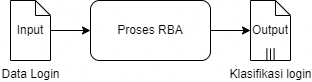
\includegraphics[width=0.6\textwidth]{contents/chapter-4/gambaran-umum.png}
    \caption{Gambaran Umum Sistem}
    \label{fig:gambaran-umum}
\end{figure}
Gambar \ref{fig:gambaran-umum} menjelaskan secara umum system bekerja dengan menggunakan metadata login sebagai input untuk mengidentifikasi risiko dari suatu transaksi. Metadata login ini kemudian diolah dan dianalisis menggunakan metode Random Forest untuk menghasilkan prediksi risiko autentikasi dengan output nya adalah klasifikasi.

Data login menggunakan dataset yang disintesis dari lebih dari 33 juta upaya login dan sekitar 3,3 juta pengguna pada layanan online skala besar di Norwegia. Data asli dikumpulkan antara Februari 2020 dan Februari 2021.

Setelah itu dataset akan digunakan untuk proses pembuatan model klasi random forest, proses pembuatan model akan melewati tiga tahap yaitu : \textit{preprocessing}, \textit{train model}
dan prediksi dataset


\subsection{Analisis Kebutuhan Sistem}
Dalam membangun sistem ini, diperlukan analisa kebutuhan fungsional dan non-fungsional. Kebutuhan fungsional adalah kebutuhan yang berkaitan dengan fungsi-fungsi yang harus ada dalam sistem. Kebutuhan non-fungsional adalah kebutuhan yang berkaitan dengan kualitas sistem yang dibangun. Kebutuhan fungsional dan non-fungsional dapat dilihat pada bagian 4.1 dan Tabel 4.2.

\subsection{Kebutuhan Fungsional}
Kebutuhan fungsional sistem ini adalah sebagai berikut:
\begin{enumerate}
    \item Sistem dapat melakukan analisis risiko autentikasi dengan menggunakan metode Random Forest.
    \item Sistem dapat men-genrate token autentikasi dari input user id.
    \item Sistem risiko autentikasi dapat terintegrasi dengan sistem FHIR.
\end{enumerate}

\subsection{Kebutuhan Non-Fungsional}
Analisis kebutuhan non fungsional dibagi menjadi dua, yaitu analisis
kebutuhan perangkat lunak dan analisis kebutuhan perangkat keras. Analisis
perangkat keras bertujuan untuk memudahkan proses perancangan dan
implementasi dalam pembangunan sistem ini.

\subsubsection{Analisis Kebutuhan Perangkat Lunak}

\begin{enumerate}
    \item Bahasa pemrograman python versi 3.9 dengan anaconda 3
    \item Framework flask untuk membuat endpoint 
    \item Sistem operasi dengan base unix untuk menjalankan sistem klasifikasi
\end{enumerate}

\subsubsection{Analisis Kebutuhan Perangkat Keras}
\begin{enumerate}
    \item Laptop atau PC dengan RAM minimal 8gb
    \item Prosessor dengan minimum 5 CPU Core 
    \item \textit{Storage} dengan minimum 50gb
\end{enumerate}

\section{Rancangan Sistem}
Berikut adalah rancangan sistem yang akan dibangun. Rancangan sistem terdiri dari rancangan arsitektur sistem, rancangan pembersihan data, rancangan variabel kepentingan, dan rancangan integrasi dengan sistem FHIR.

\subsection{Rancangan Arsitektur Sistem}
Rancangan arsitektur sistem dapat dilihat pada Gambar \ref{fig:arsitektur-sistem}. Sistem ini terdiri dari 3 komponen utama yaitu komponen \textit{data preprocessing}, komponen \textit{data mining}, dan komponen \textit{data integration}. Komponen \textit{data preprocessing} berfungsi untuk membersihkan data dari \textit{noise} dan \textit{outlier}. Komponen \textit{data mining} berfungsi untuk melakukan analisis risiko autentikasi dengan menggunakan metode Random Forest. Komponen \textit{data integration} berfungsi untuk mengintegrasikan sistem dengan sistem FHIR.

\begin{figure}[H]
    \centering
    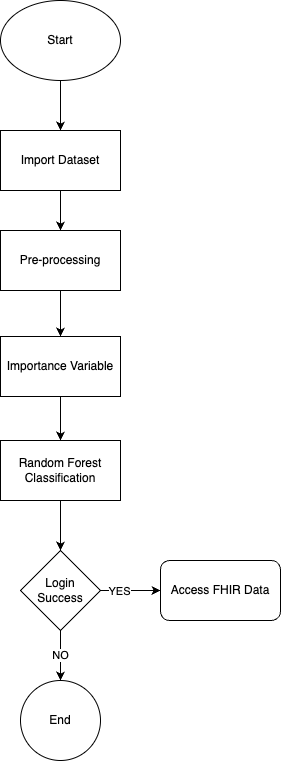
\includegraphics[width=0.5\textwidth]{contents/chapter-4/diagram-khusus.png}
    \caption{Rancangan Arsitektur Sistem}
    \label{fig:arsitektur-sistem}
\end{figure}

Pada Gambar \ref{fig:arsitektur-sistem}, sistem ini akan mendapatkan data login dari datasest. Data login ini kemudian akan digunakan sebagai input untuk melakukan analisis risiko autentikasi.

Dalam menentukan risiko autentikasi, sistem ini akan menggunakan metode Random Forest. Metode Random Forest akan menghasilkan variabel kepentingan yang dapat digunakan untuk melakukan analisis risiko autentikasi.

Setelah itu, sistem ini akan terintegrasi dengan sistem FHIR. Sistem ini akan menggunakan FHIR API untuk mengakses data dari sistem FHIR. FHIR API akan mengakses data dari sistem FHIR dengan menggunakan \textit{request} dan \textit{response}.

\subsection{Rancangan Pembersihan Data}
Rancangan pembersihan data dapat dilihat pada Gambar \ref{fig:pembersihan-data} Pada tahap ini, data akan dibersihkan dari \textit{noise} dan \textit{outlier}. \textit{Noise} adalah data yang tidak memiliki nilai yang berarti. \textit{Outlier} adalah data yang memiliki nilai yang ekstrim. Pada tahap ini, data akan dibersihkan dari \textit{noise} dan \textit{outlier} dengan menggunakan beberapa metode yaitu :

\begin{figure}[H]
    \centering
    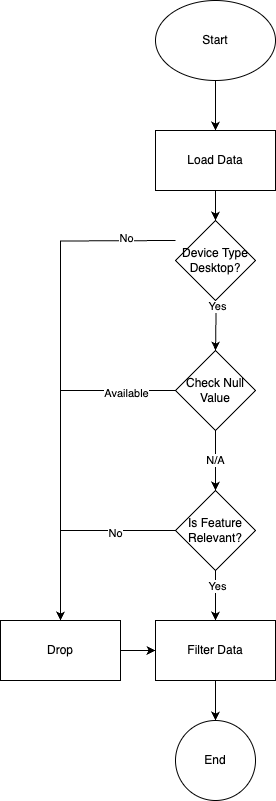
\includegraphics[width=0.4\textwidth]{contents/chapter-4/pre-processing.png}
    \caption{Rancangan Pembersihan Data}
    \label{fig:pembersihan-data}
\end{figure}

Dalam melakukan pembersihan data, sistem ini akan dua metode yaitu :

\begin{enumerate}
    \item \textit{Missing Value} : Menghapus data yang memiliki nilai kosong.
    \item \textit{Duplicate Elimination} : Menghapus duplikasi data sehingga hanya satu dari data duplikat yang disimpan. 
\end{enumerate}

Pembersihan tahap satu dapat dilakukkan menggunakan fitur pandas yaitu isnull. Setelah itu didapatkan jumlahnya dengan sum. Dengan cara ini didapatkan jumlah data kosong untuk setiap fitur. Untuk fitur yang terdapat nilai kosong akan dibuang
Pembersihan tahap dua dilakukkan dengan cara menyaring fitur \textit{User Agent and Device Type} 
Setelah data dibersihkan, data akan digunakan sebagai input untuk melakukan analisis risiko autentikasi. Data ini kemudian akan digunakan sebagai input untuk melakukan analisis risiko autentikasi.

\subsection{Rancangan Variabel Kepentingan}
Rancangan variabel kepentingan akan dilakukan dengan menggunakan metode Random Forest. Metode Random Forest akan menghasilkan variabel kepentingan yang dapat dilihat pada Gambar \ref{fig:variabel-kepentingan}. Variabel kepentingan ini akan digunakan untuk melakukan analisis risiko autentikasi.
Berikut adalah rancangan variabel kepentingan yang akan digunakan untuk melakukan analisis risiko autentikasi.
\begin{figure}[H]
    \centering
    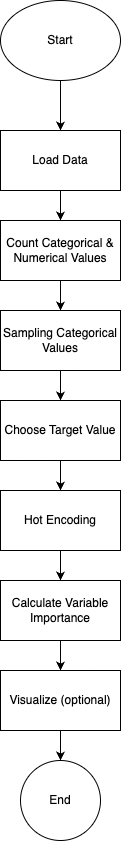
\includegraphics[width=0.2\textwidth]{contents/chapter-4/vim.drawio.png}
    \caption{Rancangan Variabel Kepentingan}
    \label{fig:variabel-kepentingan}
\end{figure}

Gambar \ref{fig:variabel-kepentingan} menjelaskan bahwa variabel kepentingan akan digunakan untuk melakukan analisis risiko autentikasi. Variabel kepentingan ini akan digunakan sebagai input untuk melakukan analisis risiko autentikasi.

Setelah data berhasil di-import akan diakukan penghitungan kategorikal dan numerikal data 

\subsection{Rancangan Integrasi Dengan Sistem FHIR}
Rancangan integrasi dengan sistem FHIR dapat dilihat pada Gambar 4.6. Sistem ini akan terintegrasi dengan sistem FHIR untuk mendapatkan data login dari pasien. Data login ini kemudian akan digunakan sebagai input untuk melakukan analisis risiko autentikasi.
\begin{figure}[H]
    \centering
    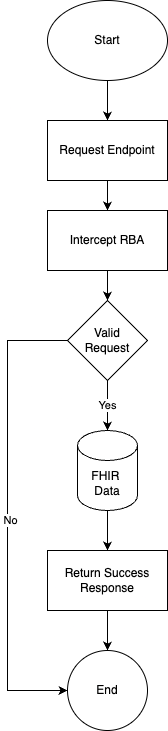
\includegraphics[width=0.2\textwidth]{contents/chapter-4/fhir-rba.drawio.png}
    \caption{Rancangan Integrasi Dengan Sistem FHIR}
    \label{fig:integrasi}
\end{figure}

Untuk melakukan integrasi dengan sistem FHIR, sistem ini akan menggunakan FHIR API. FHIR API adalah sebuah API yang digunakan untuk mengakses data dari sistem FHIR. FHIR API akan mengakses data dari sistem FHIR dengan menggunakan \textit{request} dan \textit{response}.

\section{Rancangan Pengujian}
Pengujian sistem ini akan dilakukan dengan menggunakan beberapa metode yaitu:
\begin{enumerate}
    \item Pengujian Fungsional : Pengujian fungsional dilakukan untuk menguji apakah sistem dapat berjalan dengan baik sesuai dengan kebutuhan fungsional yang telah ditentukan.
    \item Menentukan Evaluasi : Akurasi, Presisi, \textit{Recall}, \textit{F1 Score}, dan \textit{Confusion Matrix} akan digunakan untuk menentukan evaluasi dari sistem.
\end{enumerate}

\cleardoublepage \phantomsection
\chapter{IMPLEMENTASI}
Pada bab ini akan dijelaskan mengenai implementasi dari sistem yang telah dibangun. Implementasi sistem ini terdiri dari pengumpulan data, persiapan data, pemilihan fitur, dan pembangunan sistem.

\section{Pengumpulan Data}
Dalam penelitian ini data yang digunakan adalah data fitur login dari lebih dari 33 juta upaya login dan lebih dari 3,3 juta pengguna pada layanan online berskala besar di Norwegia. Data asli dikumpulkan antara Februari 2020 dan Februari 2021 dari Kaggle. Data ini berisi 284807 baris data dengan 31 kolom. Kolom-kolom tersebut adalah sebagai berikut:

\begin{longtable}{|p{0.2\textwidth}|p{0.15\textwidth}|p{0.3\textwidth}|p{0.2\textwidth}|}
    \hline
    \textbf{Feature} & \textbf{Data Type} & \textbf{Description} & \textbf{Range or Example} \\ \hline
    IP Address & String & IP address belonging to the login attempt & 0.0.0.0 - 255.255.255.255 \\ \hline
    Country & String & Country derived from the IP address & US \\ \hline
    Region & String & Region derived from the IP address & New York \\ \hline
    City & String & City derived from the IP address & Rochester \\ \hline
    ASN & Integer & Autonomous system number derived from the IP address & 0 - 600000 \\ \hline
    User Agent String & String & User agent string submitted by the client & Mozilla/5.0 (Windows NT 10.0; Win64; ... \\ \hline
    OS Name and Version & String & Operating system name and version derived from the user agent string & Windows 10 \\ \hline
    Browser Name and Version & String & Browser name and version derived from the user agent string & Chrome 70.0.3538 \\ \hline
    Device Type & String & Device type derived from the user agent string & (`mobile`, `desktop`, `tablet`, `bot`, `unknown`) \\ \hline
    User ID & Integer & Identification number related to the affected user account & Random pseudonym \\ \hline
    Login Timestamp & Integer & Timestamp related to the login attempt & 64 Bit timestamp \\ \hline
    Round-Trip Time (RTT) [ms] & Integer & Server-side measured latency between client and server & 1 - 8600000 \\ \hline
    Login Successful & Boolean & `True`: Login was successful, `False`: Login failed & (`true`, `false`) \\ \hline
    Is Attack IP & Boolean & IP address was found in known attacker data set & (`true`, `false`) \\ \hline
    Is Account Takeover & Boolean & Login attempt was identified as account takeover by incident response team of the online service & (`true`, `false`) \\ \hline
    \caption{Deskripsi tabel fitur login}
    \label{tab:my_label}
\end{longtable}

\section{Persiapan Data}
Penggunaan dataset dalam penelitian ini membutuhkan beberapa tahapan persiapan data, yaitu:

\subsection{Eksplorasi Data}
Tahap ini diperlukan untuk mendapat gambaran umum mengenai data yang digunakan. Pada tahap ini dilakukan eksplorasi data untuk mengetahui jumlah baris dan kolom, tipe data, dan statistik deskriptif dari data. Hasil eksplorasi data dapat dilihat pada Tabel 5.1.

\subsubsection{Sampling Data}
Berikut sampling data menggunakan metode random sampling dengan jumlah data 5 baris.

\begin{lstlisting}
    import pandas as pd
    
    features = pd.read_csv('data.csv')
    features.head()
    \end{lstlisting}

\subsection{Pemilihan Target}
Pada tahap ini dilakukan pemilihan target yang akan diprediksi. Sebagaimana Random Forest merupakan algoritma klasifikasi, maka penelitian ini memerlukan fitur apa yang menjadi target.

Melakukkan sampling terhadap tiga kolom yang dapat menjadi target, yaitu 'Login Successful', 'Is Attack IP', dan 'Is Account Takeover'. Berikut adalah kode untuk sampling data.

\begin{lstlisting}
    # calculate the percentage of True and False values in bolean char'
    value_counts_1 = df['is_login_success'].value_counts(normalize=True)
    is_login_success_true = value_counts_1[True] * 100
    is_login_success_false = value_counts_1[False] * 100
    print("is_login_success")
    print(f"Percentage of True values: {is_login_success_true:.2f}%")
    print(f"Percentage of False values: {is_login_success_false:.2f}%")

    value_counts_2 = df['is_attack_ip'].value_counts(normalize=True)
    is_attack_ip_true  = value_counts_2[True] * 100
    is_attack_ip_false = value_counts_2[False] * 100
    print("is_attack_ip")
    print(f"Percentage of True values: {is_attack_ip_true:.2f}%")
    print(f"Percentage of False values: {is_attack_ip_false:.2f}%")

    value_counts_3 = df['is_account_takeover'].value_counts(normalize=True)
    is_account_takeover_true  = value_counts_3[True] * 100
    is_account_takeover_false = value_counts_3[False] * 100
    print("is_account_takeover")
    print(f"Percentage of True values: {is_account_takeover_true:.2f}%")
    print(f"Percentage of False values: {is_account_takeover_false:.2f}%")
    \end{lstlisting}

    Berikut adalah hasil sampling data.

    \begin{table}[H]
        \centering
        \begin{tabular}{|l|l|l|}
        \hline
        \textbf{Target} & \textbf{True} & \textbf{False} \\ \hline
        Login Successful & 67,35\% & 32,65\% \\ \hline
        Is Attack IP & 3,09\% & 96,91\% \\ \hline
        Is Account Takeover & 0,01\% & 99,99\% \\ \hline
        \end{tabular}
        \caption{Hasil Sampling Data}
        \label{tab:sampling_data}
        \end{table}

        Dari hasil sampling data di atas, terlihat bahwa kolom 'Login Successful' memiliki persentase True yang lebih besar dibandingkan dengan False, sehingga kolom ini dipilih sebagai target.


\subsection{Pengecekan \textit{Missing Value}}
Menggunakan kode berikut untuk mengecek apakah ada nilai yang hilang pada setiap kolom.
\begin{lstlisting}
    features.isnull().sum()
    \end{lstlisting}

hasilnya adalah sebagai berikut:

\begin{table}[H]
    \centering
    \begin{tabular}{|l|l|}
    \hline
    \textbf{Feature} & \textbf{Missing Values} \\ \hline
    Index & 0 \\ 
    Login Timestamp & 0 \\ 
    User ID & 0 \\ 
    Round-Trip Time [ms] & 29993329 \\ 
    IP Address & 0 \\ 
    Country & 0 \\ 
    Region & 47409 \\ 
    City & 8590 \\ 
    ASN & 0 \\ 
    User Agent String & 0 \\ 
    Browser Name and Version & 0 \\ 
    OS Name and Version & 0 \\ 
    Device Type & 1526 \\ 
    Login Successful & 0 \\ 
    Is Attack IP & 0 \\ 
    Is Account Takeover & 0 \\ \hline
    \end{tabular}
    \caption{Missing Values in Each Feature}
    \label{tab:missing_values}
    \end{table}

Dari tabel, terlihat bahwa sebagian besar kolom tidak memiliki nilai yang hilang, namun ada juga yang memilikinya. Misalnya, kolom 'Waktu Pulang Pergi [ms]' memiliki 29993329 nilai yang hilang, kolom 'Wilayah' memiliki 47409 nilai yang hilang, kolom 'Kota' memiliki 8590 nilai yang hilang, dan kolom 'Jenis Perangkat' memiliki 1526 nilai yang hilang.

\subsection{Penambahan Kolom Token}
Kolom token dibuat untuk menyimpan token yang digunakan untuk mengakses API. Kolom ini dibuat dengan cara mengenerate token secara acak menggunakan SHA512. Berikut adalah contoh kode untuk membuat kolom token.

\begin{lstlisting}
    # generate SHA512 Hash from user_id as m2m token
    import hashlib

    def generate_sha512_hash(user_id):
        sha512_hash = hashlib.sha512()
        sha512_hash.update(str(user_id).encode('utf-8'))
        return sha512_hash.hexdigest()

    features['token'] = features['user_id'].apply(generate_sha512_hash)
    \end{lstlisting}

Berikut adalah contoh token yang digenerate.

\begin{table}[H]
    \begin{tabular}{|l|l|}
    \hline
    \textbf{User ID} & \textbf{Token} \\ \hline
    -3065936140549856249 & 4ffe29f1960c24624ec2c36909f3b39cb8d59fa18515f4 \\
    5932501938287412564 & ecee6cc95d3b047c8f796b8e772a468124b7ddb599a7a3 \\ \hline
    \end{tabular}
    \caption{Contoh Token}
    \label{tab:token}
    \end{table}

\subsection{Pembersihan Data}
Pada proses pembersihan data, dilakukan penamaan kolom, pembersihan data yang tidak diperlukan, seperti kolom 'Index' dan lainnya. Berikut adalah contoh kode untuk melakukan pembersihan data.

\subsubsection{Penamaan Kolom}
Penamaan kolom dilakukan untuk mempermudah pemanggilan kolom. Berikut adalah contoh kode untuk melakukan penamaan kolom.

\begin{lstlisting}
    # rename above columns to snake case
    features = features.rename(columns={'Login Timestamp': 'login_timestamp', 'User ID': 'user_id', 'Round-Trip Time [ms]':'round_trip','Region':'region', 'City':'city', 'ASN':'asn', 'IP Address': 'ip_address', 'Country': 'country', 'User Agent String': 'user_agent_string','Device Type': 'device_type', 'Browser Name and Version': 'browser', 'Is Account Takeover':'is_account_takeover', 'OS Name and Version':'os_detail','Login Successful':'is_login_success','Is Attack IP':'is_attack_ip'})
    \end{lstlisting}

    \begin{table}[H]
        \centering
        \begin{tabular}{|l|l|}
        \hline
        \textbf{Original Column Name} & \textbf{New Column Name} \\ \hline
        Login Timestamp & login\_timestamp \\ 
        User ID & user\_id \\ 
        Round-Trip Time [ms] & round\_trip \\ 
        Region & region \\ 
        City & city \\ 
        ASN & asn \\ 
        IP Address & ip\_address \\ 
        Country & country \\ 
        User Agent String & user\_agent\_string \\ 
        Device Type & device\_type \\ 
        Browser Name and Version & browser \\ 
        Is Account Takeover & is\_account\_takeover \\ 
        OS Name and Version & os\_detail \\ 
        Login Successful & is\_login\_success \\ 
        Is Attack IP & is\_attack\_ip \\ \hline
        \end{tabular}
        \caption{Column Renaming in DataFrame}
        \label{tab:column_renaming}
        \end{table}

\subsubsection{Penyaringan User Agent dan Device Type}
Hal ini dilakukan untuk membatasi jumlah dataset dan device type yang bertujuan mengurangi waktu komputasi dalam pembuatan model. Berikut adalah contoh kode untuk melakukan penyaringan user agent dan device type. 

\begin{lstlisting}
    # check lenght in column user_agent_string
    features['length'] = features['user_agent_string'].apply(
        lambda row: min(len(row), len(row)) if isinstance(row, str) else None
    )
    print(features['length'].mean())
    \end{lstlisting}

    Kode di atas digunakan untuk mengetahui panjang rata-rata string pada kolom 'User Agent String'. Hasilnya adalah 136.652141700553. 
    Setelah itu dilakukan penyaringan data dengan cara menghapus data yang memiliki panjang string lebih dari 136. Berikut adalah contoh kode untuk melakukan penyaringan data.

\begin{lstlisting}
    # only keep rows with device type desktop
    features = features[features.device_type == 'desktop']
    # filter the DataFrame based on the length of column 'user_agent_string'
    features = features[features['user_agent_string'].str.len() < 136]
    \end{lstlisting}

    Setelah itu dilakukan penyaringan data dengan cara menghapus data yang memiliki device type selain 'desktop'.

\subsection{Menghapus Kolom yang Tidak Diperlukan}
Pada tahap ini dilakukan penghapusan kolom yang tidak diperlukan. Kolom yang dihapus adalah kolom 'Round-Trip Time [ms]', 'Index', 'Is Attack IP', 'Is Account Takeover', 'User ID', 'Token', 'Device Type', dan 'Length'. Berikut adalah contoh kode untuk menghapus kolom yang tidak diperlukan.

\begin{lstlisting}
    # drop unsued columns
    features = features.drop(['round_trip', 'index', 'is_attack_ip', 'is_account_takeover', 'user_id', 'token', 'device_type', 'length'], axis=1, inplace=True)
    \end{lstlisting}

Hasil keluaran dari tahap ini adalah sebagai berikut. 

\begin{table}[H]
    \centering
    \begin{tabular}{|l|l|l|l|}
    \hline
    \textbf{Column Name} & \textbf{Data Type} & \textbf{\#Distinct} & \textbf{NA Values} \\ \hline
    login\_timestamp & object & 30000 & 0 \\ 
    ip\_address & object & 17387 & 0 \\ 
    country & object & 75 & 0 \\ 
    region & object & 273 & 14 \\ 
    city & object & 1414 & 7 \\ 
    asn & int64 & 792 & 0 \\ 
    user\_agent\_string & object & 637 & 0 \\ 
    browser & object & 167 & 0 \\ 
    os\_detail & object & 61 & 0 \\ 
    is\_login\_success & bool & 2 & 0 \\ \hline
    \end{tabular}
    \caption{Revised Initial Exploratory Data Analysis}
    \label{tab:revised_initial_eda}
    \end{table}

    Berdasarkan tabel di atas, diperoleh 30000 data, dengan 10 kolom, dan ada 14 data yang memiliki nilai kosong pada kolom 'Region' dan 7 data yang memiliki nilai kosong pada kolom 'City'.


\section{Implementasi Pemilihan Fitur}
Pada bagian ini akan dijelaskan mengenai implementasi pemilihan fitur. Pemilihan fitur dilakukan dengan cara memilih fitur yang memiliki korelasi tinggi dengan target. Berikut adalah tahapan pemilihan fitur.

\subsubsection{Eksplorasi Tipe Data}
Tahap ini diperlukan untuk mengetahui tipe data dari setiap kolom. Asumsi yang digunakan adalah kolom yang memiliki tipe data numerik memiliki korelasi yang lebih tinggi dibandingkan dengan kolom yang memiliki tipe data string.
Berikut adalah contoh kode untuk mengetahui tipe data dari setiap kolom.

\begin{lstlisting}
    categorical = [var for var in df.columns if df[var].dtype=='O']
    print('There are {} categorical variables\n'.format(len(categorical)))
    print('The categorical variables are :\n\n', categorical)

    There are 8 categorical variables

    The categorical variables are :
    ['login_timestamp', 'ip_address', 'country', 'region', 'city', 'user_agent_string', 'browser', 'os_detail']
    \end{lstlisting}

    Berikut adalah hasil keluaran dari tahap ini.

    \begin{table}[H]
        \centering
        \begin{tabular}{|l|l|}
        \hline
        \textbf{Column Name} & \textbf{Data Type} \\ \hline
        login\_timestamp & object \\ 
        ip\_address & object \\ 
        country & object \\ 
        region & object \\ 
        city & object \\ 
        asn & int64 \\ 
        user\_agent\_string & object \\ 
        browser & object \\ 
        os\_detail & object \\ 
        is\_login\_success & bool \\ \hline
        \end{tabular}
        \caption{Data Type of Each Column}
        \label{tab:data_type}
        \end{table}

        Berdasarkan tabel di atas, terlihat bahwa kolom 'ASN' memiliki tipe data numerik, sedangkan kolom lainnya memiliki tipe data string.


\subsection{Encoding}
Berdasarkan tabel di atas, terlihat bahwa kolom 'ASN' memiliki tipe data numerik, sedangkan kolom lainnya memiliki tipe data string. Oleh karena itu, perlu dilakukan encoding terhadap kolom-kolom yang memiliki tipe data string. Berikut adalah contoh kode untuk melakukan encoding.

\begin{lstlisting}
    import category_encoders as ce

    # One-hot encode the categorical features
    # encode categorical variables with ordinal encoding
    # see def preprocess_data(df) above
    encoder = ce.OneHotEncoder(cols= ['login_timestamp', 'ip_address', 'country', 'region', 'city', 'user_agent_string', 'browser', 'os_detail'])
    X_train = encoder.fit_transform(X_train)
    
    X_test = encoder.transform(X_test)
    X_train.head()
    \end{lstlisting}

    Berikut adalah hasil keluaran dari tahap ini.

\subsection{Gini Importance}
Setelah dilakukan encoding, maka seluruh kolom memiliki tipe data numerik. Berikut adalah contoh kode untuk melakukan pemilihan fitur menggunakan Gini Importance.

\begin{lstlisting}
    ### Gini importance 
    # create the classifier with n_estimators = default
    clf = RandomForestClassifier(random_state=0)

    # fit the model to the training set
    clf.fit(X_train, y_train)

    # view the feature scores
    feature_scores = pd.Series(clf.feature_importances_, index=X_train.columns).sort_values(ascending=False)
    
    # Top 10 important features
    feature_scores.head(10) 
    \end{lstlisting}

    Pada kode di atas dilakukan pemilihan 10 fitur teratas. Dikarenakan jumlah fitur yang banyak, setelah dilakukkan encoding maka akan sulit untuk memvisualisasikan seluruh fitur.
    Berikut adalah hasil keluaran dari tahap ini.

    \begin{table}[H]
    \centering
    \begin{tabular}{|l|l|}
    \hline
    \textbf{Feature} & \textbf{Gini Importance} \\ \hline
    asn & 0.017551 \\ 
    country\_2 & 0.009943 \\ 
    country\_4 & 0.004708 \\ 
    country\_6 & 0.003670 \\ 
    ip\_address\_23 & 0.003618 \\ 
    os\_detail\_1 & 0.003317 \\ 
    browser\_1 & 0.002975 \\ 
    os\_detail\_16 & 0.002832 \\ 
    user\_agent\_string\_49 & 0.002508 \\ 
    browser\_2 & 0.002213 \\ \hline
    \end{tabular}
    \caption{Gini Importance of Each Feature}
    \label{tab:gini_importance}
    \end{table}

    Dalam tabel di atas, jika di lakukkan pengelompokkan maka akan terlihat bahwa fitur 'asn', 'country', 'ip\_address', 'os\_detail', 'browser', dan 'user\_agent\_string' memiliki nilai Gini Importance yang tinggi. 
    Namun, hanya 4 group teratas yang memiliki nilai Gini Importance yang tinggi, yaitu 'asn', 'country', 'ip\_address', dan 'os\_detail' yang akan digunakan sebagai fitur dalam pembuatan model.

\section{Pembuatan Random Forest}
Pada bagian ini akan dijelaskan mengenai implementasi pembuatan Random Forest. Pembuatan Random Forest dapat dilakukan setelah memilih fitur yang memiliki korelasi tinggi dengan target. Berikut adalah tahapan pembuatan Random Forest.
Dari proses eksplorasi tipe data tabel 5.7 dan 5.2.2 pemilihan target, maka diperoleh bahwa kolom 'Login Successful' memiliki korelasi yang tinggi dengan target. Oleh karena itu, kolom ini dipilih sebagai target.
\subsection{Pembagian Data}
Pada tahap ini dilakukan pembagian data meliputi

\subsubsection{Pembagian Data Fitur dan Target}
Pada tahap ini dilakukan pembagian data fitur dan target. Berikut adalah contoh kode untuk melakukan pembagian data fitur dan target.
\begin{lstlisting}
    # Separate the features (X) and the target (y)
    X = df_encoded.drop(columns=['is_login_success'])
    y = df_encoded['is_login_success']
    \end{lstlisting}

    Kode di atas digunakan untuk memisahkan fitur dan target. Fitur disimpan pada variabel X, sedangkan target disimpan pada variabel y.

\subsubsection{Pembagian Data Training dan Data Testing}
Pada tahap ini dilakukan pembagian data training dan data testing. Berikut adalah contoh kode untuk melakukan pembagian data training dan data testing.
\begin{lstlisting}
    # Split the data into training and test sets
    X_train, X_test, y_train, y_test = train_test_split(X, y, test_size = 0.3, random_state=42)
\end{lstlisting}

    Kode di atas digunakan untuk membagi data menjadi data training dan data testing. Data training disimpan pada variabel X\_train dan y\_train, sedangkan data testing disimpan pada variabel X\_test dan y\_test.
    Set pelatihan digunakan untuk melatih model, dan set pengujian digunakan untuk mengevaluasi performa model pada data yang tidak terlihat. 
    Fungsi train\_test\_split dari modul sklearn.model\_selection digunakan untuk melakukan ini. Parameter test\_size disetel ke 0,3, artinya 30\% data akan digunakan untuk set pengujian, dan sisanya 70\% akan digunakan untuk set pelatihan. Parameter random\_state disetel ke 42 untuk memastikan bahwa pemisahan yang dihasilkan dapat direproduksi.

\subsection{Pembuatan Model dan Pelatihan Model}
Pada tahap ini dilakukan pembuatan model. Berikut adalah contoh kode untuk melakukan pembuatan model.
\begin{lstlisting}
    # Create the classifier with n_estimators = 0
    clf = RandomForestClassifier(random_state=0)

    # Fit the model to the data
    clf.fit(X_train, y_train)
\end{lstlisting}
    
Kode Python yang dipilih ini menginisialisasi dan melatih klasifikasi Random Forest. Berikut adalah penjelasannya:

\begin{enumerate}
\item \textbf{Menginisialisasi klasifikasi Random Forest:} Baris 
2 membuat instance baru dari klasifikasi Random Forest. Parameter \texttt{random\_state} diatur ke 0 untuk reproduktibilitas. Ini berarti bahwa pemisahan yang dihasilkan dapat direproduksi, yang penting untuk hasil yang konsisten di berbagai penjalanan.
\item \textbf{Melatih klasifikasi Random Forest:} Baris ke 5 melatih klasifikasi Random Forest pada data latihan. Metode \texttt{fit} menerima dua argumen: fitur (\texttt{X\_train}) dan target (\texttt{y\_train}). Fitur adalah input untuk model, dan target adalah apa yang ingin kita prediksi dari model.
\end{enumerate}

Kelas \texttt{RandomForestClassifier} memiliki banyak parameter yang dapat disesuaikan untuk mengoptimalkan kinerja model. Dalam kasus ini, hanya parameter \texttt{random\_state} yang diatur, dan semua parameter lain dibiarkan sebagai nilai default.

\subsection{Evaluasi Model}
Pada tahap ini dilakukan evaluasi model. Berikut adalah contoh kode untuk melakukan evaluasi model.
\begin{lstlisting}
    # Make predictions on the test set
    y_pred = clf.predict(X_test)
    
    # Evaluate the accuracy of the model
    accuracy = accuracy_score(y_test, y_pred)
    print('Accuracy:', accuracy)
    
    # Calculate precision, recall, and F1 score
    precision = precision_score(y_test, y_pred)
    recall = recall_score(y_test, y_pred)
    f1 = f1_score(y_test, y_pred)
    
    print('Precision:', precision)
    print('Recall:', recall)
    print('F1 Score:', f1)
\end{lstlisting}

Kode di atas digunakan untuk melakukan evaluasi model. Berikut adalah penjelasannya:
Tahap ini mengevaluasi kinerja model machine learning menggunakan beberapa metrik: akurasi, presisi, recall, dan skor F1. Berikut adalah penjelasannya:

\begin{enumerate}
\item \textbf{Evaluasi Akurasi:} Beberapa baris pertama menghitung akurasi prediksi model. Akurasi adalah proporsi prediksi yang benar dari semua prediksi. Ini adalah metrik umum untuk masalah klasifikasi. Fungsi \texttt{accuracy\_score} dari \texttt{sklearn.metrics} digunakan untuk menghitung akurasi. Hasilnya dicetak ke konsol.
\item \textbf{Menghitung Presisi, Recall, dan Skor F1:} Sisa kode menghitung presisi, recall, dan skor F1 dari prediksi model. Ini adalah metrik umum lainnya untuk masalah klasifikasi.
   \begin{itemize}
   \item Presisi adalah proporsi prediksi positif benar dari semua prediksi positif. Ini adalah ukuran berapa banyak prediksi positif yang sebenarnya benar.
   \item Recall (juga dikenal sebagai sensitivitas) adalah proporsi prediksi positif benar dari semua positif aktual. Ini adalah ukuran berapa banyak instansi positif aktual yang dapat diidentifikasi model.
   \item Skor F1 adalah rata-rata harmonik dari presisi dan recall. Ini memberikan skor tunggal yang menyeimbangkan kedua kekhawatiran presisi dan recall dalam satu angka.
   \end{itemize}
\end{enumerate}

Metrik ini dihitung menggunakan fungsi \texttt{precision\_score}, \texttt{recall\_score}, dan \texttt{f1\_score} dari \texttt{sklearn.metrics}, masing-masing. Hasilnya kemudian dicetak ke konsol.

\subsection{Visualisasi Model}
Pada tahap ini dilakukan visualisasi model. Berikut adalah contoh kode untuk melakukan visualisasi model.
\begin{lstlisting}
    # Visualize a single decision tree
    plt.figure(figsize=(12,12))
    tree = plot_tree(clf.estimators_[0], feature_names=X.columns, filled=True, rounded=True, fontsize=10)
    \end{lstlisting}

    Kode di atas digunakan untuk melakukan visualisasi model. Berikut adalah penjelasannya:
    Tahap ini memvisualisasikan satu pohon keputusan dari model Random Forest. Ini memberikan gambaran tentang bagaimana model membuat prediksi. Berikut adalah penjelasannya:

    \begin{enumerate}
    \item \textbf{Menginisialisasi plot:} Baris 2 menginisialisasi plot dengan ukuran 12 x 12 inci. Ini memastikan bahwa plot cukup besar untuk ditampilkan dengan jelas.
    \item \textbf{Membuat plot:} Baris 3 membuat plot menggunakan fungsi \texttt{plot\_tree} dari \texttt{sklearn.tree}. Ini mengambil tiga argumen: model (\texttt{clf.estimators\_[0]}), nama fitur (\texttt{X.columns}), dan beberapa parameter untuk mengontrol penampilan plot. Hasilnya adalah plot pohon keputusan.
    \end{enumerate}

    % \begin{figure}[H]
    %     \centering
    %     \includegraphics[width=0.8\textwidth]{img/decision_tree.png}
    %     \caption{Decision Tree}
    %     \label{fig:decision_tree}
    %     \end{figure}

        Gambar 5.1 menunjukkan plot pohon keputusan. Setiap node dalam pohon mewakili satu aturan yang digunakan untuk membuat prediksi. Pada node akar, model memeriksa apakah nilai fitur 'asn' lebih kecil dari 0,5. Jika iya, maka model akan memprediksi bahwa pengguna tidak berhasil login. Jika tidak, maka model akan memeriksa apakah nilai fitur 'asn' lebih kecil dari 1,5. Jika iya, maka model akan memprediksi bahwa pengguna berhasil login. Jika tidak, maka model akan memeriksa apakah nilai fitur 'asn' lebih kecil dari 2,5. Jika iya,
        

\section{Pembagunan Sistem}
Sistem dibangun berbasis API dengan menggunakan bahasa pemrograman Python 3.9.13 . Sistem ini menggunakan beberapa library, yaitu:
1. Anaconda 3 versi 2022.10 untuk mengatur lingkungan kerja Python.
2. Flask versi 2.0.2 untuk membuat API.
3. Pandas versi 1.3.4 untuk memanipulasi data.
4. Scikit-learn versi 1.0 untuk membangun model.
5. Pickle versi 4.0 untuk menyimpan model.
6. Algoritma SHA512 untuk membuat token.
7. Pytest versi 6.2.5 untuk melakukan testing.

\subsection{Pembangunan API}





\cleardoublepage \phantomsection
\chapter{HASIL DAN PEMBAHASAN}
Pada bagian ini dijelaskan mengenai hasil dari penelitian yang telah dilakukan. Penjelasan dibagi menjadi beberapa bagian, yaitu hasil pengujian, analisis hasil pengujian, dan pembahasan hasil pengujian.

\section{Hasil Pengujian}
Hasil pengujian berupa hasil pengujian fungsional, hasil pengujian non-fungsional, hasil pengujian eksperimental, dan hasil pengujian lainnya. Hasil pengujian fungsional berisi hasil pengujian terhadap fitur-fitur yang ada pada sistem. Hasil pengujian non-fungsional berisi hasil pengujian terhadap aspek non-fungsional yang ada pada sistem. Hasil pengujian eksperimental berisi hasil pengujian terhadap sistem yang dibandingkan dengan sistem lainnya. Hasil pengujian lainnya berisi hasil pengujian yang tidak termasuk dalam hasil pengujian fungsional, non-fungsional, dan eksperimental.

\subsection{Kinerja Sistem}
Hasil pengujian kinerja sistem berisi hasil pengujian terhadap kinerja sistem. Pengujian kinerja sistem dilakukan dengan cara mengukur waktu yang dibutuhkan oleh sistem untuk menyelesaikan suatu proses. Pengujian kinerja sistem dilakukan dengan cara membandingkan waktu yang dibutuhkan oleh sistem untuk menyelesaikan suatu proses dengan waktu yang dibutuhkan oleh sistem lainnya untuk menyelesaikan proses yang sama.

\subsubsection{Waktu Data Training}
Hasil pengujian waktu data training berisi hasil pengujian terhadap waktu yang dibutuhkan oleh sistem untuk melakukan proses data training. Pengujian ini dilakukan dengan cara membandingkan waktu yang dibutuhkan oleh sistem untuk melakukan proses data training.
Dalam pengujian ini, dilakukkan pengujian untuk beberapa ukuran dataset. Ukuran dataset yang digunakan adalah 10000, 20000, 30000, 40000 dan 50000. 
Berikut adalah hasil pengujian waktu data training.

\begin{table}[H]
    \centering
    \begin{tabular}{|c|c|}
    \hline
    \textbf{Ukuran Dataset} & \textbf{Waktu Data Training (detik)} \\
    \hline
    10000 & 453 \\
    \hline
    20000 & 901 \\
    \hline
    30000 & 1937 \\
    \hline
    40000 & 2237 \\
    \hline
    50000 & error \\
    \hline
    \end{tabular}
    \caption{Hasil Pengujian Waktu Data Training}
    \label{table:1}
\end{table}


\subsubsection{Penggunaan Memori dan CPU}
Hasil pengujian penggunaan memori dan CPU berisi hasil pengujian terhadap penggunaan memori dan CPU oleh sistem. Pengujian ini dilakukan dengan cara membandingkan penggunaan memori dan CPU.

\begin{table}[H]
    \centering
    \begin{tabular}{|c|c|c|}
    \hline
    \textbf{Ukuran Dataset} & \textbf{Penggunaan CPU (\%)} & \textbf{Memory Usage (MB)} \\
    \hline
    10000 & 5 & 600 \\
    \hline
    20000 & 9,2 & 701 \\
    \hline
    30000 & 14 & 722 \\
    \hline
    40000 & 18,5 & 729 \\
    \hline
    \end{tabular}
    \caption{Hasil Pengujian Penggunaan CPU dan Memory Data Training}
    \label{table:1}
\end{table}


\subsection{Performa Sistem}
Hasil pengujian performa sistem berisi hasil pengujian terhadap performa sistem. Pengujian performa sistem dilakukan dengan cara membandingkan performa sistem dengan performa sistem lainnya.
\subsubsection{Pengujian Random Forest}
Hasil pengujian random forest berisi hasil pengujian terhadap random forest. Pada pengujian pertama ingin dilihat bagaimana performa random forest dengan menggunakan beberapa parameter yang berbeda. Pada pengujian kedua ingin dilihat bagaimana performa random forest dengan menggunakan parameter yang telah dioptimasi.
Dalam percobaan ini dipilih 4 parameter yang akan dioptimasi, yaitu: max\_depth, min\_samples\_leaf, min\_samples\_split, dan n\_estimators. Untuk setiap parameter, akan dicoba beberapa nilai yang berbeda. Untuk setiap kombinasi parameter, akan dilakukan 5 kali percobaan. Untuk setiap percobaan, akan dilakukan 5 kali validasi silang. Dengan demikian, total percobaan yang dilakukan adalah 5 x 5 x 5 x 5 = 625 percobaan.

\begin{table}[h]
    \centering
    \begin{tabular}{|c|c|}
    \hline
    \textbf{Parameter} & \textbf{Values} \\
    \hline
    n\_estimators & 100, 200, 500 \\
    \hline
    max\_depth & None, 10, 20 \\
    \hline
    min\_samples\_split & 2, 5, 10 \\
    \hline
    min\_samples\_leaf & 1, 2, 4 \\
    \hline
    \end{tabular}
    \caption{Parameter Grid}
    \label{table:param_grid}
    \end{table}

Pada Tabel \ref{table:param_grid} ditunjukkan hasil pengujian random forest dengan menggunakan beberapa parameter yang berbeda. Pada tabel \ref{table:sampel_hasil_pengujian_random_forest} ditunjukkan sampel hasil pengujian random forest dengan menggunakan parameter yang telah dioptimasi.


\begin{table}[h]
    \centering
    \begin{tabularx}{\textwidth}{|X|c|c|c|c|}
    \hline
    \textbf{Parameters} & \textbf{Accuracy} & \textbf{Precision} & \textbf{Recall} & \textbf{F1 Score} \\
    \hline
    \{'max\_depth': None, 'min\_samples\_leaf': 1, 'min\_samples\_split': 2, 'n\_estimators': 100\} & 0.668 & 0.737 & 0.788 & 0.762 \\
    \hline
    \{'max\_depth': None, 'min\_samples\_leaf': 1, 'min\_samples\_split': 2, 'n\_estimators': 200\} & 0.669 & 0.739 & 0.790 & 0.763 \\
    \hline
    % ... add the rest of your rows here ...
    \{'max\_depth': None, 'min\_samples\_leaf': 4, 'min\_samples\_split': 2, 'n\_estimators': 500\} & 0.708 & 0.701 & 0.968 & 0.813 \\
    \hline
    \end{tabularx}
    \caption{Model Parameters and Performance Metrics}
    \label{table:sampel_hasil_pengujian_random_forest}
\end{table}

Tabel \ref{table:sampel_hasil_pengujian_random_forest} adalah hasil pengujian random forest dengan menggunakan parameter yang telah dioptimasi. Ditemukan bahwa parameter yang menghasilkan performa terbaik adalah \{'max\_depth': None, 'min\_samples\_leaf': 2, 'min\_samples\_split': 2, 'n\_estimators': 200\} dengan akurasi 0.708, presisi 0.701, recall 0.968, dan F1 score 0.813.

\section{Analisis Hasil Pengujian}
Analisis hasil pengujian berisi analisis terhadap hasil pengujian yang telah dilakukan. Analisis dilakukan dengan membandingkan hasil pengujian dengan spesifikasi kebutuhan yang telah ditetapkan sebelumnya. Apabila hasil pengujian sesuai dengan spesifikasi kebutuhan, maka sistem dapat dikatakan berhasil. Sebaliknya, apabila hasil pengujian tidak sesuai dengan spesifikasi kebutuhan, maka sistem dapat dikatakan gagal.
Dalam melakukan analisis hasil pengujian, dapat digunakan beberapa metode, yaitu:
Confusion Matrix: Implementasi confusion matrix membantu memahami sejauh mana model dapat mengidentifikasi True Positives (mesin yang diakui dengan benar), True Negatives (mesin yang ditolak dengan benar), False Positives (mesin yang salah diakui), dan False Negatives (mesin yang salah ditolak).

\begin{figure}
    \centering
    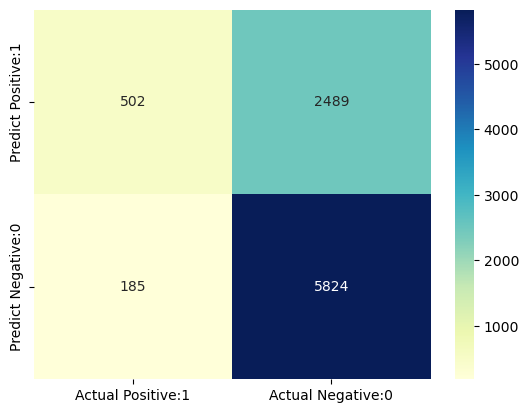
\includegraphics[width=0.5\textwidth]{contents/chapter-6/confusion_matrix.png}
    \caption{Confusion Matrix}
    \label{fig:confusion_matrix}
\end{figure}

\begin{table}[H]
    \centering
    \begin{tabular}{|c|c|c|}
    \hline
     & \textbf{Predicted: 0} & \textbf{Predicted: 1} \\
    \hline
    \textbf{Actual: 0} & True Negative & False Positive \\
    \hline
    \textbf{Actual: 1} & False Negative & True Positive \\
    \hline
    \end{tabular}
    \caption{Confusion Matrix}
    \label{table:1}
\end{table}

Hasil tertinggi yang diperoleh dari Tabel \ref{table:sampel_hasil_pengujian_random_forest} adalah sebagai berikut:

\begin{table}[H]
    \centering
    \begin{tabular}{|c|c|}
    \hline
    \textbf{Parameter} & \textbf{Values} \\
    \hline
    n\_estimators & 500 \\
    \hline
    max\_depth & None \\
    \hline
    min\_samples\_split & 2 \\
    \hline
    min\_samples\_leaf & 2 \\
    \hline
    \end{tabular}
    \caption{Hasil Pengujian Random Forest}
    \label{table:2}
    \end{table}

Dengan hasil sebagai akurasi 0.708, presisi 0.701, recall 0.968, dan F1 score 0.813. Dengan hasil ini diperoleh akurasi yang lebih rendah dari yang diharapkan. Hal ini disebabkan oleh dataset yang digunakan tidak seimbang. Dengan demikian, model yang dihasilkan cenderung memprediksi kelas mayoritas. Untuk membuktikan hal ini, dapat dilakukan pengecekan dengan melihat presentase target pada dataset. Berikut adalah presentase target pada dataset

\begin{figure}[H]
    \centering
    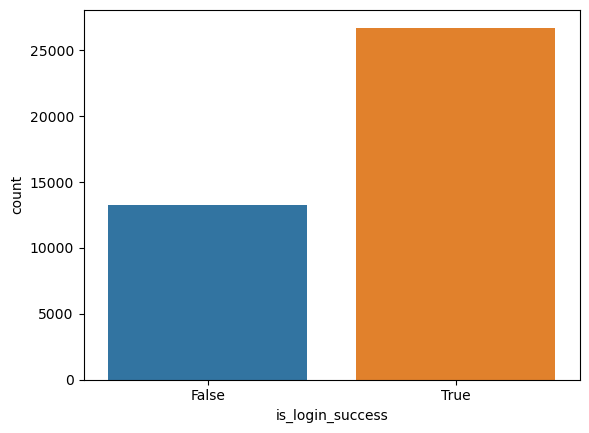
\includegraphics[width=0.5\textwidth]{contents/chapter-6/visualize_class.png}
    \caption{Presentase Target pada Dataset}
    \label{fig:visualize_target}
\end{figure}

Berdasarkan Gambar \ref{fig:visualize_target}, dapat dilihat bahwa presentase target pada dataset adalah 0.5. Dengan demikian, dapat disimpulkan bahwa dataset yang digunakan tidak seimbang. Menurut (Sun dkk., 2009) dataset yang digunakan tidak seimbang dapat menyebabkan model yang dihasilkan cenderung memprediksi kelas mayoritas. Hal ini menyebabkan akurasi yang dihasilkan lebih rendah dari yang diharapkan.





\section{Pembahasan Hasil Pengujian}
Pembahasan hasil pengujian berisi pembahasan terhadap hasil pengujian yang telah dilakukan. Pembahasan dilakukan dengan membandingkan hasil pengujian dengan spesifikasi kebutuhan yang telah ditetapkan sebelumnya. Apabila hasil pengujian sesuai dengan spesifikasi kebutuhan, maka sistem dapat dikatakan berhasil. Sebaliknya, apabila hasil pengujian tidak sesuai dengan spesifikasi kebutuhan, maka sistem dapat dikatakan gagal.

\cleardoublepage \phantomsection
\chapter{KESIMPULAN DAN SARAN}
Pada bagian ini dijelaskan mengenai kesimpulan dari penelitian yang telah dilakukan. Penjelasan dibagi menjadi beberapa bagian, yaitu kesimpulan, dan saran.

\section{Kesimpulan}
Kesimpulan dari penelitian ini adalah sebagai berikut:
\begin{enumerate}
    \item Model yang dihasilkan belum dapat mengklasifikasi risiko autentikasi dengan baik. Sistem autentikasi M2M berbasis risiko menggunakan Random Forest dapat mengklasikasi risiko autentikasi. Dengan akurasi 70.8\%, presisi 70.1\%, \textit{recall} 96.8\%, dan \textit{F1-score} 71.3\%. Ketimpangan akurasi dan \textit{recall} disebabkan oleh ketidakseimbangan jumlah data pada kelas yang berbeda.
    \item Pembatasan fitur kepentingan dapat berpengaruh pada akurasi sistem.
\end{enumerate}


\section{Saran}
Penelitian ini masih memiliki beberapa kekurangan yang dapat diperbaiki pada penelitian selanjutnya, yaitu:
\begin{enumerate}
    \item Penelitian ini masih menggunakan dataset hybrid. Sehingga perlu dilakukan penelitian lebih lanjut dengan menggunakan dataset asli.
    \item Akurasi sistem masih dapat ditingkatkan, serta perlu dilakukan penelitian lebih lanjut untuk meningkatkan keamanan sistem.
    \item Opitimasi parameter Random Forest masih dapat dilakukan lebih lanjut.
    \item Dapat dilakukan perbandingan dengan memilih target parameter yang berbeda.
\end{enumerate}


%======================================

%======================================
%  References
%======================================
\cleardoublepage \phantomsection
\thereferences
% You can change 
%    the filename and location of the files inputted
\bibliography{references}

%Hapus bagian di bawah setelah tidak diperlukan

%======================================

%======================================
%  Appendix
%======================================
% You can change 
%    the filename and location of the files inputted
%    use \chapterappendix for the first page of the appendix
%    use \chapterappendixadd for the next page

\appendix

\cleardoublepage \phantomsection
% \chapterappendix{contents/appendix/appendix-isi-lampiran}
% \chapterappendixadd{contents/appendix/appendix-latex}
% \chapterappendixadd{contents/appendix/appendix-penulisan-referensi}
% \chapterappendixadd{contents/appendix/appendix-code}




%======================================

\end{document}